\documentclass[10pt, twocolumn]{IEEEtran}

\usepackage{bm}
\usepackage{url}
\usepackage{bbm}
\usepackage{cite}
\usepackage{array}
\usepackage{ifthen}
\usepackage{xspace}
\usepackage{dsfont}
\usepackage{siunitx}
\usepackage{amsmath}
\usepackage{amssymb}
\usepackage{multicol}
\usepackage{amsfonts}
\usepackage{mathrsfs}
\usepackage{booktabs}
\usepackage{graphicx}
\usepackage{caption}
\usepackage{setspace}
\usepackage{hyperref}
\usepackage{makecell}
\usepackage{footnote}
\usepackage{verbatim}
\usepackage{algorithm}
\usepackage{subcaption}
\usepackage{glossaries}
\usepackage{soul,xcolor}
\usepackage[T1]{fontenc}
\usepackage{algpseudocode}
\usepackage{algcompatible}
\usepackage[normalem]{ulem}
\usepackage{multirow,enumitem}

\captionsetup{font=footnotesize}

\renewcommand\theadalign{c}
\renewcommand\theadfont{\bfseries}
\renewcommand\cellgape{\Gape[2pt]}
\renewcommand\theadgape{\Gape[2pt]}

\newcommand{\tot}{\mathrm{tot}}
\newcommand{\numberthis}{\addtocounter{equation}{1}\tag{\theequation}}

\sisetup{detect-all,range-phrase=--,range-units=single}
\newcommand\mst[2][red]{\setbox0=\hbox{$#2$}\rlap{\raisebox{.45\ht0}{\textcolor{#1}{\rule{\wd0}{2pt}}}}#2}

\setlength{\textfloatsep}{1.5pt}
\newcommand{\tfrm}{T_{\mathrm{fr}}}
\newcommand{\beam}[1]{\mathcal B_{#1}}
\newcommand{\size}[1]{\left | #1 \right|}
\newcommand{\bk}[1]{\textcolor{blue}{[BK: #1]}}
\newcommand{\yz}[1]{\textcolor{blue}{[YZ: #1]}}
\newcommand{\ca}[1]{\textcolor{magenta}{[CA: #1]}}
\newcommand{\nm}[1]{\textcolor{magenta}{[NM: #1]}}
\newcommand{\beambs}[1]{\mathcal B_{{\mathrm t},#1}}
\newcommand{\beamue}[1]{\mathcal B_{{\mathrm r},#1}}
\newcommand{\diag}[1]{\mathrm{diag}\left(#1 \right)}

\newcommand{\sst}[1]{\st{#1}}
\newcommand{\prob}{\mathbb{P}}
\newcommand{\tfr}{T_{\mathrm{fr}}}
\newcommand{\vect}[1]{\mathbf{#1}}
\newcommand{\wtot}{W_{\mathrm{tot}}}
\newcommand{\add}[1]{\textcolor{red}{#1}}

\DeclareMathOperator{\Exp}{\mathbb{E}}
\DeclareMathOperator*{\argmax}{arg\,max}
\DeclareMathOperator*{\argmin}{arg\,min}

\title{Propagation Measurements and Analyses at \SI{28}{\giga\hertz} via an Autonomous Beam-Steering Platform}
\author{\vspace{-1mm}Bharath Keshavamurthy\IEEEauthorrefmark{1}, Yaguang Zhang\IEEEauthorrefmark{2}, Christopher R. Anderson\IEEEauthorrefmark{3},\\Nicol\`{o} Michelusi\IEEEauthorrefmark{1}, James V. Krogmeier\IEEEauthorrefmark{2}, and David J. Love\IEEEauthorrefmark{2}
\thanks{\IEEEauthorrefmark{1}Electrical, Computer and Energy Engineering, Arizona State University.}
\thanks{\IEEEauthorrefmark{2}Electrical and Computer Engineering, Purdue University.}
\thanks{\IEEEauthorrefmark{3}Electrical Engineering, United States Naval Academy.}
\thanks{A summary of this research was presented at URSI NRSM 2022 \cite{NRSM}.}
\thanks{Research funded by NSF under grants CNS-1642982 and CNS-2129615.}
\thanks{Source code is available on \href{https://github.com/bharathkeshavamurthy/SPAVE-28G.git}{GitHub}\cite{SPAVE-28G-Software}. Dataset is available on \href{https://doi.org/10.5281/zenodo.7178597}{Zenodo}\cite{SPAVE-28G-Dataset}.}
\vspace{-10mm}
}

\begin{document}
\bstctlcite{IEEEexample:BSTcontrol}

\maketitle
\thispagestyle{plain}
\pagestyle{plain}
\setulcolor{red}
\setul{red}{2pt}
\setstcolor{red}
\vspace{-10mm}

\begin{abstract}
We detail the design of an autonomous alignment and tracking platform for mechanically steering directional horn antennas in a sliding correlator channel sounder setup for \SI{28}{\giga\hertz} V$2$X propagation modeling on the NSF POWDER testbed. A pan-and-tilt subsystem facilitates uninhibited rotational mobility along the yaw and pitch axes, driven by open-loop servo units, orchestrated via inertial motion controllers. Deploying a rooftop mounted transmitter and a mobile receiver driven around onsite, a geo-positioning subsystem augmented in accuracy by RTK streams enables navigation events to be shared between the two over a fault-tolerant Apache Kafka publish-subscribe framework. Herein, we demonstrate a $3$D geo-positioning accuracy of \SI{17}{\centi\meter}, an average principal axes positioning accuracy of \SI{1.1}{\degree} across all yaw and pitch movements, and an average tracking response time of \SI{27.8}{\milli\second}. Leveraging commercial off-the-shelf components, this cost-effective design also mitigates the need for exhaustive signal sampling strategies inherent in electronic beam-steering systems. The power-delay profiles, collected along routes spanning urban and suburban environments, are used in pathloss evaluations involving macro-cellular ITU and $3$GPP models. Crucially, fully autonomous antenna alignment operations allow for continuous tracking and measurement, which uniquely permits millimeter wave channel modeling in vehicular settings. With the SAGE algorithm for multi-path component extraction, in addition to RMS delay- and direction-spread analyses, we perform signal decoherence studies vis-\`{a}-vis distance, alignment, and velocity.
% CRA, YZ: What insights did you gain from the decoherence studies?
\end{abstract}
\vspace{-1mm}

\begin{IEEEkeywords}
Millimeter Wave, Beam Alignment, V$2$X
\end{IEEEkeywords}
\vspace{-5mm}

\section{Introduction}\label{S1}
The widespread adoption and recent acceleration in the deployment of $5$G networks has resulted in an increased strain on the mid-band spectrum (\SIrange{4}{8}{\giga\hertz}), thereby causing providers around the world to shift their spectrum focus onto the millimeter wave bands \cite{Commercial}. Concurrently, with mmWave deployments, both consumers and businesses can exploit the relatively higher bandwidth over extant mid-band networks: consumers can experience better quality-of-service vis-\`{a}-vis data rates at their user terminals, while businesses can leverage reliable service guarantees to optimize operations \cite{Rappaport, UCSB}. 

While mmWave networks deliver quality-of-service gains, the signals suffer from poor propagation characteristics, i.e., increased atmospheric attenuation and absorption \cite{Rappaport}. Ergo, there have been concerted efforts from both academia and industry to develop well-rounded mmWave channel models in indoor and outdoor environments \cite{Indoor60G, QDC, NISTModeling, MacCartneyUrbanHumanBlockage}. Current efforts comprise a wide array of propagation modeling campaigns and subsequent analyses---however, they suffer from limitations in system design \cite{Agile-Link, Harvard}; fail to address diversity in transmitter (Tx) and receiver (Rx) deployment \cite{Purdue, MolischSpatialOutdoor}; rarely evaluate the collected pathloss behavior against standardized models \cite{Outdoor28G, Commercial}; and involve semi-stationary measurements \cite{Qualcomm3GPP, CapacityEvaluation} that neglect signal decoherence studies under continuously varying Tx-Rx distance, alignment, and relative velocity.

To address these limitations, we employ a sliding correlator channel sounder \cite{Sounder} in conjunction with a fully autonomous robotic beam-steering platform, as part of a V$2$X propagation modeling campaign on the NSF POWDER testbed \cite{POWDER} in urban and suburban environments at \SI{28}{\giga\hertz}.  Measurements were used to perform pathloss analyses incorporating outdoor macro-cellular ITU and $3$GPP standards \cite{MacCartneyModelsOverview, Qualcomm3GPP}, delay- and direction-spread studies, and signal decorrelation behavior.

This paper makes several important contributions.  First, our propagation modeling campaign on POWDER involves greater deployment diversity owing to our data collection activities along routes in both urban and suburban settings (location diversity); under manual, full-, and semi-autonomous alignment operations (beam-steering diversity); and using heterogeneous mobile mounts (vehicle vs cart, velocity diversity). In contrast, the \SI{28}{\giga\hertz} measurement campaign in \cite{Purdue} centers around a manual antenna alignment platform in suburban neighborhoods under semi-stationary settings only; the sampling activities in \cite{Harvard} are constrained to indoor environments and the underlying beam-steering platform also requires manual operation; and \cite{MolischSpatialOutdoor, Outdoor28G} outline semi-stationary approaches restricted to urban deployments. Second, while electronic beam-alignment systems \cite{Agile-Link} involving phased-array antenna modules offer increased flexibility in side-lobe \& beam-width control and demonstrate faster average tracking response times (${\approx}$\SI{2.5}{\milli\second} vs \SI{27.8}{\milli\second}) relative to mechanical fixed-beam steering, they constitute exhaustive beam-search strategies and their design necessitates expensive hardware to host inherently resource-heavy algorithms. Additionally, our work evaluates the collected measurements against the $3$GPP TR$38.901$ and ITU-R M$.2135$ large-scale macro-cellular pathloss models \cite{MacCartneyModelsOverview, Qualcomm3GPP}.  These comparisons enable us to gain novel insights on adapting them to rapidly evolving mmWave V$2$V and V$2$I scenarios \cite{5GFastMovingVehicles, V2IMeasurements}. Lastly, while \cite{MolischEstimate, MolischSpatialIndoorOutdoor, MolischSpatialOutdoor, MacCartneySpatialStatistics} conduct spatial consistency analyses of mmWave signals with respect to Tx-Rx distance, they fail to investigate signal decorrelation behavior under real-time variations in Tx-Rx alignment and relative velocity. With a fully autonomous beam-alignment platform that aids in the steady and continual series of measurements along random vehicular routes, our design facilitates spatial decoherence studies under alignment and relative velocity variations. The insights gathered from these studies on mmWave signal propagation in vehicular settings can be leveraged in the efficient design and deployment of $5$G+ networks along interstates \cite{TMobileHighways, 5GADASKorea} and in furthering spatial consistency research in V$2$V and V$2$I networks \cite{MacCartneyModelsOverview}.

\indent{The} rest of the paper is organized as: Sec. \ref{S2} elucidates the end-to-end design of our autonomous mechanical beam-steering platform; Sec. \ref{S3} details our measurement and post-processing activities; Sec. \ref{S4} describes our numerical evaluations and insights gained from pathloss and spatial consistency studies; finally, Sec. \ref{S5} lists our conclusions.
\vspace{-3mm}

\section{Measurement System Description}\label{S2}
With the objective of facilitating uninterrupted data collection operations for \SI{28}{\giga\hertz} propagation modeling in V$2$X settings, our measurement campaign on the NSF POWDER testbed \cite{POWDER} involved a sliding correlator channel sounder \cite{Sounder} with directional horn antennas in conjunction with a fully autonomous mechanical beam-steering platform for continual antenna alignment and tracking \cite{NRSM}. Specifically, under V$2$I evaluations, with a rooftop mounted transmitter and a mobile receiver traversing random vehicular routes onsite, this design enables the logging of geo-positioning data (i.e., GPS location coordinates, speed, acceleration, heading), alignment values, and power-delay profile samples. Accompanied by the system architecture illustration in Fig. \ref{F1}, in this section, we first briefly discuss our sounder design and then describe the development of our antenna alignment and tracking platform.
\begin{table} [tb]
	\centering
	\scriptsize
	\begin{tabular}{|l||l|}
		\hline
		V$2$X & Vehicle-to-Vehicle (V$2$V) or Vehicle-to-Infrastructure (V$2$I)\\
		\hline
		$3$GPP TR38.901 UMa & $3$rd Generation Partnership Project (Urban Macrocells)\\
		\hline
		ITU-R M$.2135$ UMa & International Telecommunication Union (Urban Macrocells)\\
		\hline
		HPBW, SDR & Half-Power Beam-Width, Software Defined Radio\\
		\hline
		GNSS, GPS & Global Navigation Satellite System, Global Positioning System\\
		\hline
		SAGE & Space Alternating Expectation Maximization\\
		\hline
		NMEA-0183 & National Marine Electronics Association (data specification)\\
		\hline
		RTK & Real-Time Kinematics (GPS corrections)\\
		\hline
		RTCM & Radio Technical Commission for Maritime Services\\
		\hline
		NTRIP & Networked Transport of RTCM over Internet Protocol\\
		\hline
		UNAVCO & University NAVstar COnsortium (GNSS data provisioning)\\
		\hline
		SSD, SBC & Solid State Drive, Single Board Computer\\
		\hline
		NTP & Network Time Protocol (timing synchronization)\\
		\hline
		PWM & Pulse Width Modulation (digital control of servos)\\
		\hline
		I$2$C & Inter Integrated Circuit (serial communication bus)\\
		\hline
	\end{tabular}
	\vspace{-0.25mm}
	\caption{Glossary of Notations, Standards, and Protocols}
	\label{T1}
\end{table}

\noindent{\textbf{Channel Sounder}}: The measurement system employed a custom broadband sliding correlator channel sounder at both the Tx and the Rx \cite{Purdue}, each equipped with a Pseudorandom Noise (PN) sequence generator module producing the required known apriori signal for time-dilated cross-correlation studies, with the Rx module clocked at a slightly lower rate than the Tx \cite{Sounder}; up-/down-converter to transition between the \SI{2.5}{\giga\hertz} and \SI{28}{\giga\hertz} regimes; a vertically polarized directional horn antenna; and other commercially available components. This setup is depicted by the schematics in Fig. \ref{F1} and is implemented by the circuits shown in Fig. \ref{F2}. The operational specifications of our channel sounder are listed in Table \ref{T2}: the WR-$28$ directional horn antennas demonstrate $+$\SI{22}{\deci\bel{i}} gain and \SI{15}{\degree} HPBW; for all measurements, the PN code involves \SI{11}{}-bit sequences of length \SI{2047}; and the maximum measurable pathloss is estimated to be \SI{182}{\decibel}, as detailed in \cite{Purdue}. At the receiver, complex-\SI{64}{} I/Q power-delay profiles are recorded onboard an SSD-drive by a GNURadio sink on a Raspberry Pi SBC via a USRP B$200$mini SDR.

\noindent{\textbf{Alignment \& Tracking}}: First, to enable uninhibited rotational mobility for alignment and tracking in the horizontal and the vertical planes, as shown in Fig. \ref{F1}, at both the Tx and the Rx, the WR-$28$ antenna is mounted on a PT-$2645$S open-loop pan-and-tilt unit, driven by $2{\times}$ HSR-$2645$CRH continuous rotation servos, each actuating either yaw (horizontal) or pitch (vertical) alignment. These servos are controlled via PWM signals from an ATMega$328$P microcontroller with the angular position (absolute and relative) feedback provided by a BNO$080$ inertial motion unit. This principal axes positioning subsystem demonstrates an average accuracy of \SI{1.1}{\degree} across all fine- \& coarse-grained yaw and pitch movements. Next, for seamless operations in V$2$X scenarios, the alignment platform is augmented with a geo-positioning subsystem consisting of a UBlox ZED-F$9$P GPS unit (with a GNSS multi-band antenna) wherein the positioning accuracy is enhanced by RTCM v$3.0$ RTK correction streams over NTRIP from a UNAVCO caster via a Lefebure client. Demonstrating an average $3$D accuracy of \SI{17}{\centi\meter}, the relevant data members captured by this geo-positioning unit---namely, the coordinate (latitude, longitude, and ellipsoidal altitude), the horizontal speed \& acceleration, and the heading, are communicated to the microcontroller as NMEA-0183 messages using the I$2$C protocol.
\begin{table} [tb]
	\centering
	\scriptsize
	\begin{tabular}{|l||l|}
		\hline
		Carrier Frequency & \SI{28}{\giga\hertz}\\
		\hline
		PN Chip Sequence Length & \SI{2047}{}\\
		\hline
		RF Bandwidth & \SI{800}{\mega\hertz}\\
		\hline
		Tx Chip Rate & \SI{400}{\mega{cps}}\\
		\hline
		Temporal Resolution & \SI{2.5}{\nano\second}\\
		\hline
		Rx Chip Rate & \SI{399.95}{\mega{cps}}\\
		\hline
		Tx Power & \SI{23}{\deci\bel{m}}\\
		\hline
		Tx/Rx Antenna Gain & \SI{22}{\deci\bel{i}}\\
		\hline
		Measured Tx/Rx Azimuth HPBW & \SI{10.1}{\degree}\\
		\hline
		Measured Tx/Rx Elevation HPBW & \SI{11.5}{\degree}\\
		\hline
		Maximum Measurable Path Loss & \SI{182}{\decibel}\\
		\hline
		GNURadio Sink Center Frequency & \SI{2.5}{\giga\hertz}\\
		\hline
		GNURadio Sink Bandwidth & \SI{0}{\hertz}\\
		\hline
		USRP Gain & \SI{0}{\decibel} or \SI{76}{\decibel}\\
		\hline
		USRP Sampling Rate & \SI{2}{\mega{sps}}\\
		\hline
	\end{tabular}
	\vspace{0.25mm}
	\caption{Sliding Correlator Channel Sounder Specifications}
	\label{T2}
\end{table}

Since our measurement system revolves around a decoupled design with the alignment and tracking platform replicated at both the Tx and the Rx, a centralized nerve-center handles asynchronous module registration \& de-registration via RPyC object proxying \cite{RPyC}, global timing synchronization via NTP, and coordination between the Tx and Rx over fault-tolerant Apache Kafka messaging middleware. With Zookeeper broker management \cite{Kafka}, the samples generated by the principal axes positioning and geo-positioning subsystems are shared over Kafka topics: the Tx subscribes to the alignment and geo-location messages published by the Rx, and vice-versa, resulting in a scalable event-driven modular architecture. Corroborated both onsite and in the laboratory, this publish-subscribe framework facilitates an average beam-steering response time of \SI{27.8}{\milli\second}, evaluated over \SI{12,870}{} interactions. With system monitoring provided over an android debug bridge and system troubleshooting enabled via serial communication interfaces, our platform demonstrates remote orchestration capabilities: a critical necessity for V$2$X propagation modeling. Finally, to enhance remote monitoring and troubleshooting of our system, a GNURadio Qt GUI time-sink (with dynamic trigger levels) allows for real-time visualization of the recorded power-delay profiles over an ad-hoc WLAN with the Raspberry Pi SBC; additionally, via the Plotly Dash and MapBox APIs, the Tx and Rx geo-locations are annotated with their relative alignment accuracies and visualized in real-time at a control terminal for onsite validation of the routes traversed on POWDER.
\begin{figure*} [t]
    \centerline{
    \includegraphics[width=1.0\textwidth]{figs/System_Architecture.pdf}}
    \vspace{-2mm}
    \caption{The architecture of our autonomous antenna alignment \& tracking platform with a sliding correlator channel sounder.}
    \label{F1}
    \vspace{-6mm}
\end{figure*}
\vspace{-3mm}

\section{Measurements \& Post-Processing}\label{S3}
In this section, we discuss the operations involved in our \SI{28}{\giga\hertz} V$2$X measurement campaign on the POWDER testbed. First, we describe the system calibration process to establish a relationship between the USRP voltage readings (in \SI{}{\volt}) and the received signal power (in \SI{}{\deci\bel}); next, we outline the onsite system deployment procedure; and finally, we detail the post-processing steps involved in setting up the recorded samples for pathloss and spatial consistency studies.

\noindent{\textbf{Pre-deployment Calibration}}: After the Tx and Rx circuits for the sliding correlator channel sounder have been implemented as illustrated in Figs. \ref{F2}(a) and \ref{F2}(d), a calibration procedure is carried out onsite to map the power calculated from the power-delay profiles recorded by the USRP to reference measured power levels. Calibrating the measurement system before deployment ensures accurate Rx power calculations in the presence of imperfect circuit components, e.g., the Commscope LDF$4$-$50$A \SI{0.5}{{"}} coaxial cables employed at the Tx exhibit losses of up to \SI{0.12}{\deci\bel\per\meter} at \SI{2.5}{\giga\hertz}. Fig. \ref{F1} depicts the components and connections involved in setting up this calibration process. Under \SI{0}{\deci\bel} and \SI{76}{\deci\bel} USRP gains, employing a Keysight variable attenuator, the power-delay profiles collected via the GNURadio USRP sink are processed to determine the calculated power values mapped to the reference measured power levels. This procedure yields a linear relationship between the calculated and measured power values (in \SI{}{\deci\bel}), which is studied in further detail in Sec. \ref{S4}.

\noindent{\textbf{POWDER Deployment}}: As described in Sec. \ref{S2}, our measurement system assembly constitutes an autonomous beam-steering controller replicated at both the Tx and the Rx, their respective sounder circuits, and a centralized nerve center for aggregation (RPyC), synchronization (NTP), and coordination (Kafka-Zookeeper). On the POWDER testbed, first, the nerve center is deployed on a high-availability cluster of four Dell R$740$ compute nodes at the Fort Douglas datacenter---provisioned via geni-lib/RSpec scripts---with fault-tolerance being a necessary feature to ensure storage redundancy for the recorded data; next, as depicted in Fig. \ref{F2}(b), the Tx is fixed atop the rooftop of the William Browning Building; and lastly, as shown in Fig. \ref{F2}(c), the Rx is mounted on a Toyota Sienna minivan (or a push-cart) that is driven (or pushed) along random routes onsite. Remote monitoring and troubleshooting capabilities are provided at the Tx and the Rx: these enable the real-time verification of geo-positioning data, alignment accuracies, and power-delay profile records.

The goal of this measurement campaign was to obtain a reasonably large dataset of site-specific signal propagation characteristics for evaluating the propagation characteristics of \SI{28}{\giga\hertz} signals in vehicular communication settings. Thus, our propagation modeling activities included V$2$I measurements under manual, semi-, and fully-autonomous alignment operations traversing nine routes spanning both urban and suburban neighborhoods. The collected dataset ($\approx$\SI{400}{\giga{B}}) is then subjected to post-processing to visualize the received power maps along the traversed routes (see \cite{NRSM}); evaluate pathloss results against the ITU M$.2135$ and $3$GPP TR$38.901$ models \cite{MacCartneyModelsOverview, Qualcomm3GPP}; and via the SAGE algorithm \cite{SAGE1}, gather insights on the spatial decoherence behavior of mmWave signals under distance, alignment, and velocity effects.

\noindent{\textbf{Post-Processing}}: Using GNURadio utilities, the metadata file corresponding to the route-specific power-delay profile records at the Rx is parsed to extract timestamp information, which is then associated with the geo-positioning and alignment logs at both the Tx and the Rx. The samples in each synchronized power-delay profile segment undergoes pre-filtering via a low-pass filter (SciPy FIR implementation), time-windowing, and noise-elimination (via custom peak-search and thresholding heuristics). Coupled with known transmission power and antenna gain values, the received power levels obtained from these processed samples allow the visualization of pathloss maps on the Google Maps API (rendered via the Bokeh toolbox), and the evaluation of pathloss behavior as a function of Tx-Rx distance, with validations against ITU and $3$GPP standards. Using a custom implementation of the SAGE algorithm to extract the attenuation and delay parameters of multi-path components arriving at the Rx, as detailed in Sec. \ref{S4}, we study the signal spatial consistency behavior in V$2$X scenarios, in addition to RMS delay- and direction-spread analyses.
\begin{figure*}[t]
    \begin{tabular}{cc}
        \begin{minipage}{0.522\linewidth} 
        	\centering
            \includegraphics[width=1.0\linewidth]{figs/Tx_Comm_Setup_I.jpg}
            \\ [0.5ex]
            \centering
            \includegraphics[width=1.0\linewidth]{figs/Rx_Comm_Setup_I.jpg}
        \end{minipage}&
        \hspace{-5mm}
        \begin{minipage}{0.478\linewidth}
        	\centering
            \includegraphics[width=1.0\linewidth]{figs/Tx_Deployment_Browning.jpg}
            \\ [0.5ex]
            \centering
            \includegraphics[width=1.0\linewidth]{figs/Rx_Cart_Deployment.JPEG}
        \end{minipage}
    \end{tabular}
    \caption{Clockwise from top-left: The Tx circuit with a \SI{28}{\giga\hertz} up-converter, a WR-$28$ directional horn antenna, and other commercially available parts (a); The deployment of the Tx atop the William Browning building: the sounder circuits are housed in a climate-controlled enclosure with the antenna mounted on the pan-and-tilt platform (b); The deployment of the Rx mounted on a push-cart (or a minivan) and pushed (or driven) around onsite (c); The Rx circuit with a \SI{28}{\giga\hertz} down-converter, a WR-$28$ directional horn antenna, USRP B$200$mini SDR, Raspberry Pi SBC, and other commercially available parts (d).}
    \label{F2}
    \vspace{-6mm}
\end{figure*}

\section{Numerical Evaluations}\label{S4}
\vspace{-2mm}
In this section, we outline the results of our evaluations on the collected dataset. First, as shown in Fig. \ref{F3}(a), under \SI{0}{\deci\bel} and \SI{76}{\deci\bel} USRP gain values, we determine the relationship between the received power calculated from the recorded power-delay profiles during the calibration procedure and the reference measured power levels. For a specific route, upon processing the samples in each power-delay profile segment, these calibration curves are used to map the computed power to its corresponding reference measured value in order to ensure accurate analyses in the presence of lossy circuit components. Second, Figs. \ref{F3}(b) and \ref{F3}(c) depict the normalized azimuth and elevation patterns of the WR-$28$ directional horn antennas used in this campaign. Next, Fig. \ref{F4} illustrates the pathloss heatmaps superimposed on Google Hybrid maps of the routes traversed by the Rx onsite, with the Tx affixed on the rooftop of the William Browning building. Also, we compare the pathloss versus distance behavior of signals in our measurement campaign with outdoor macro-cellular pathloss standards (ITU M$.2135$ and $3$GPP TR$38.901$ \cite{MacCartneyModelsOverview, Qualcomm3GPP}). 
\begin{figure*} [t]
     \begin{subfigure}{0.333\linewidth}
         \centering
         \includegraphics[width=1.0\linewidth]{figs/Calibration_Curves.png}
         \caption{Calibration curves}
         \label{F3a}
     \end{subfigure}
     \begin{subfigure}{0.333\linewidth}
         \centering
         \includegraphics[width=1.0\linewidth]{figs/Antenna_Pattern_Normalized_2D_Azimuth.png}
         \caption{Normalized Antenna Pattern (Azimuth)}
         \label{F3b}
     \end{subfigure}
     \begin{subfigure}{0.333\linewidth}
         \centering
         \includegraphics[width=1.0\linewidth]{figs/Antenna_Pattern_Normalized_2D_Elevation.png}
         \caption{Normalized Antenna Pattern (Elevation)}
         \label{F3c}
     \end{subfigure}
     \vspace{-2mm}
     \caption{The calibration curves depicting measured power versus calculated power for USRP gains of \SI{0}{\deci\bel} and \SI{76}{\deci\bel} (a); and the normalized $2$D antenna patterns along the azimuth and elevation directions for the WR-$28$ horn antennas used in our channel sounder (b), (c).}
     \label{F3}
     \vspace{-4mm}
\end{figure*}
\begin{figure*} [t]
     \begin{subfigure}{0.333\linewidth}
         \centering
         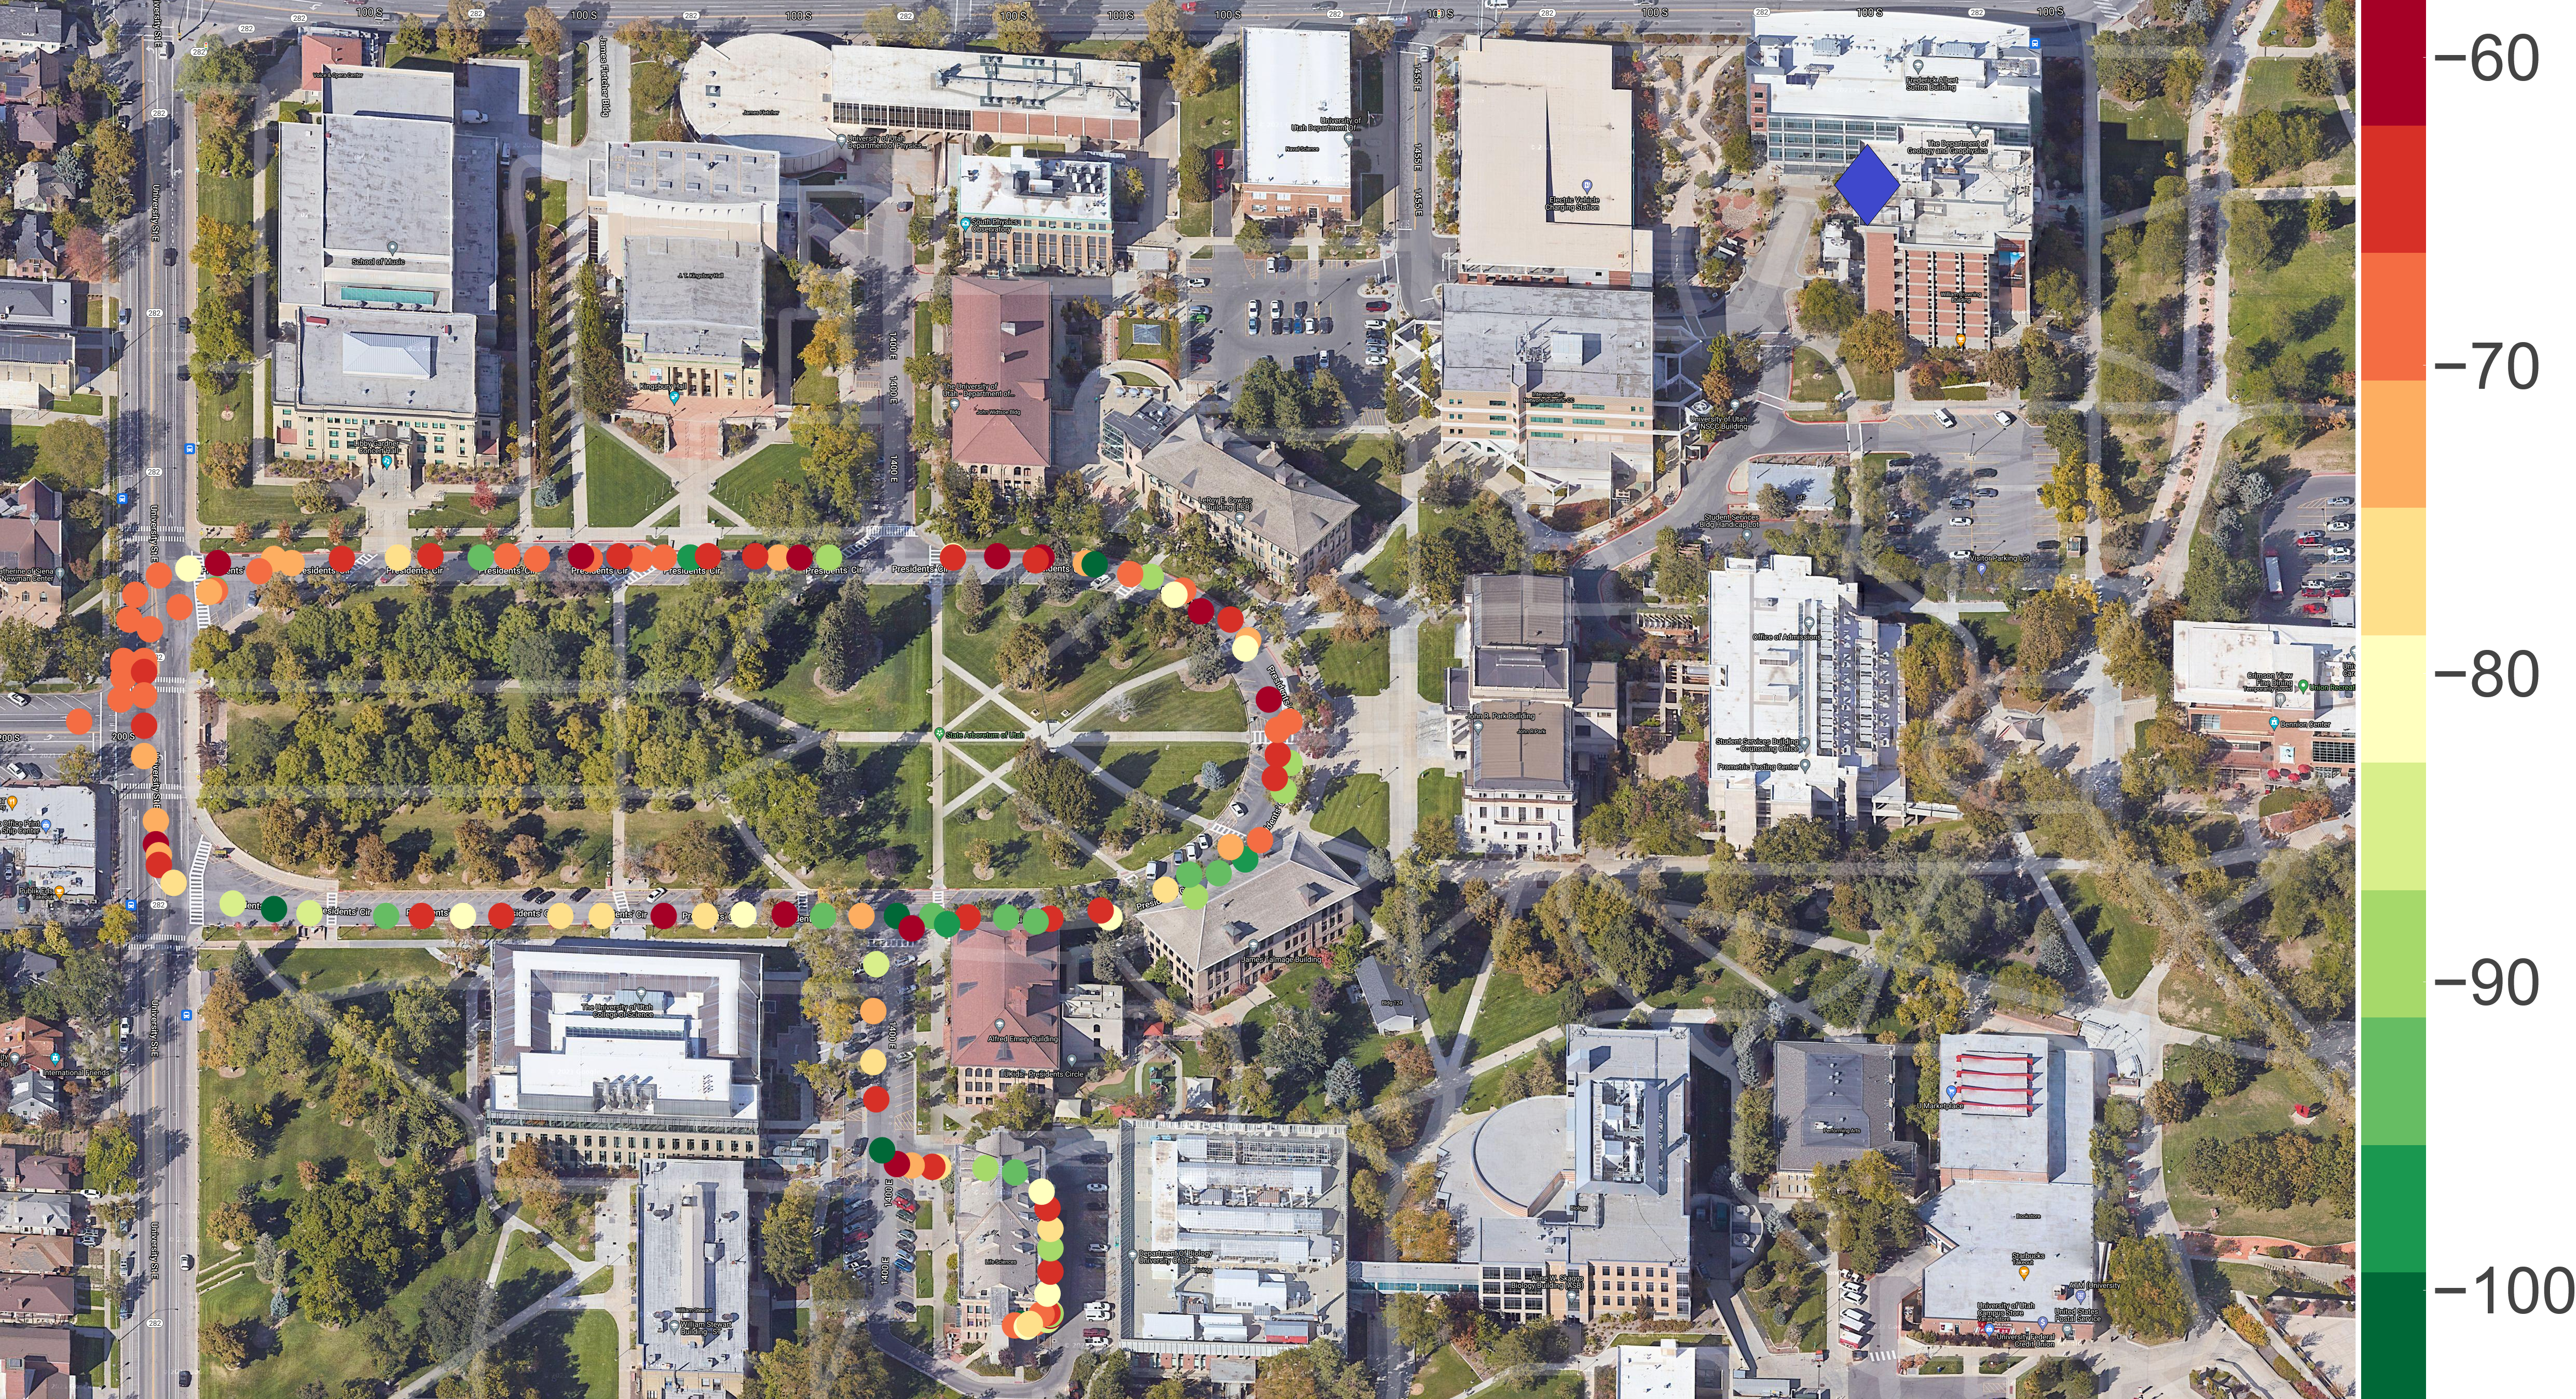
\includegraphics[width=1.0\linewidth]{figs/Rx_Power_Map_Urban_Campus.png}
         \caption{Urban Campus (President's Circle)}
         \label{F4a}
     \end{subfigure}
     \begin{subfigure}{0.333\linewidth}
         \centering
         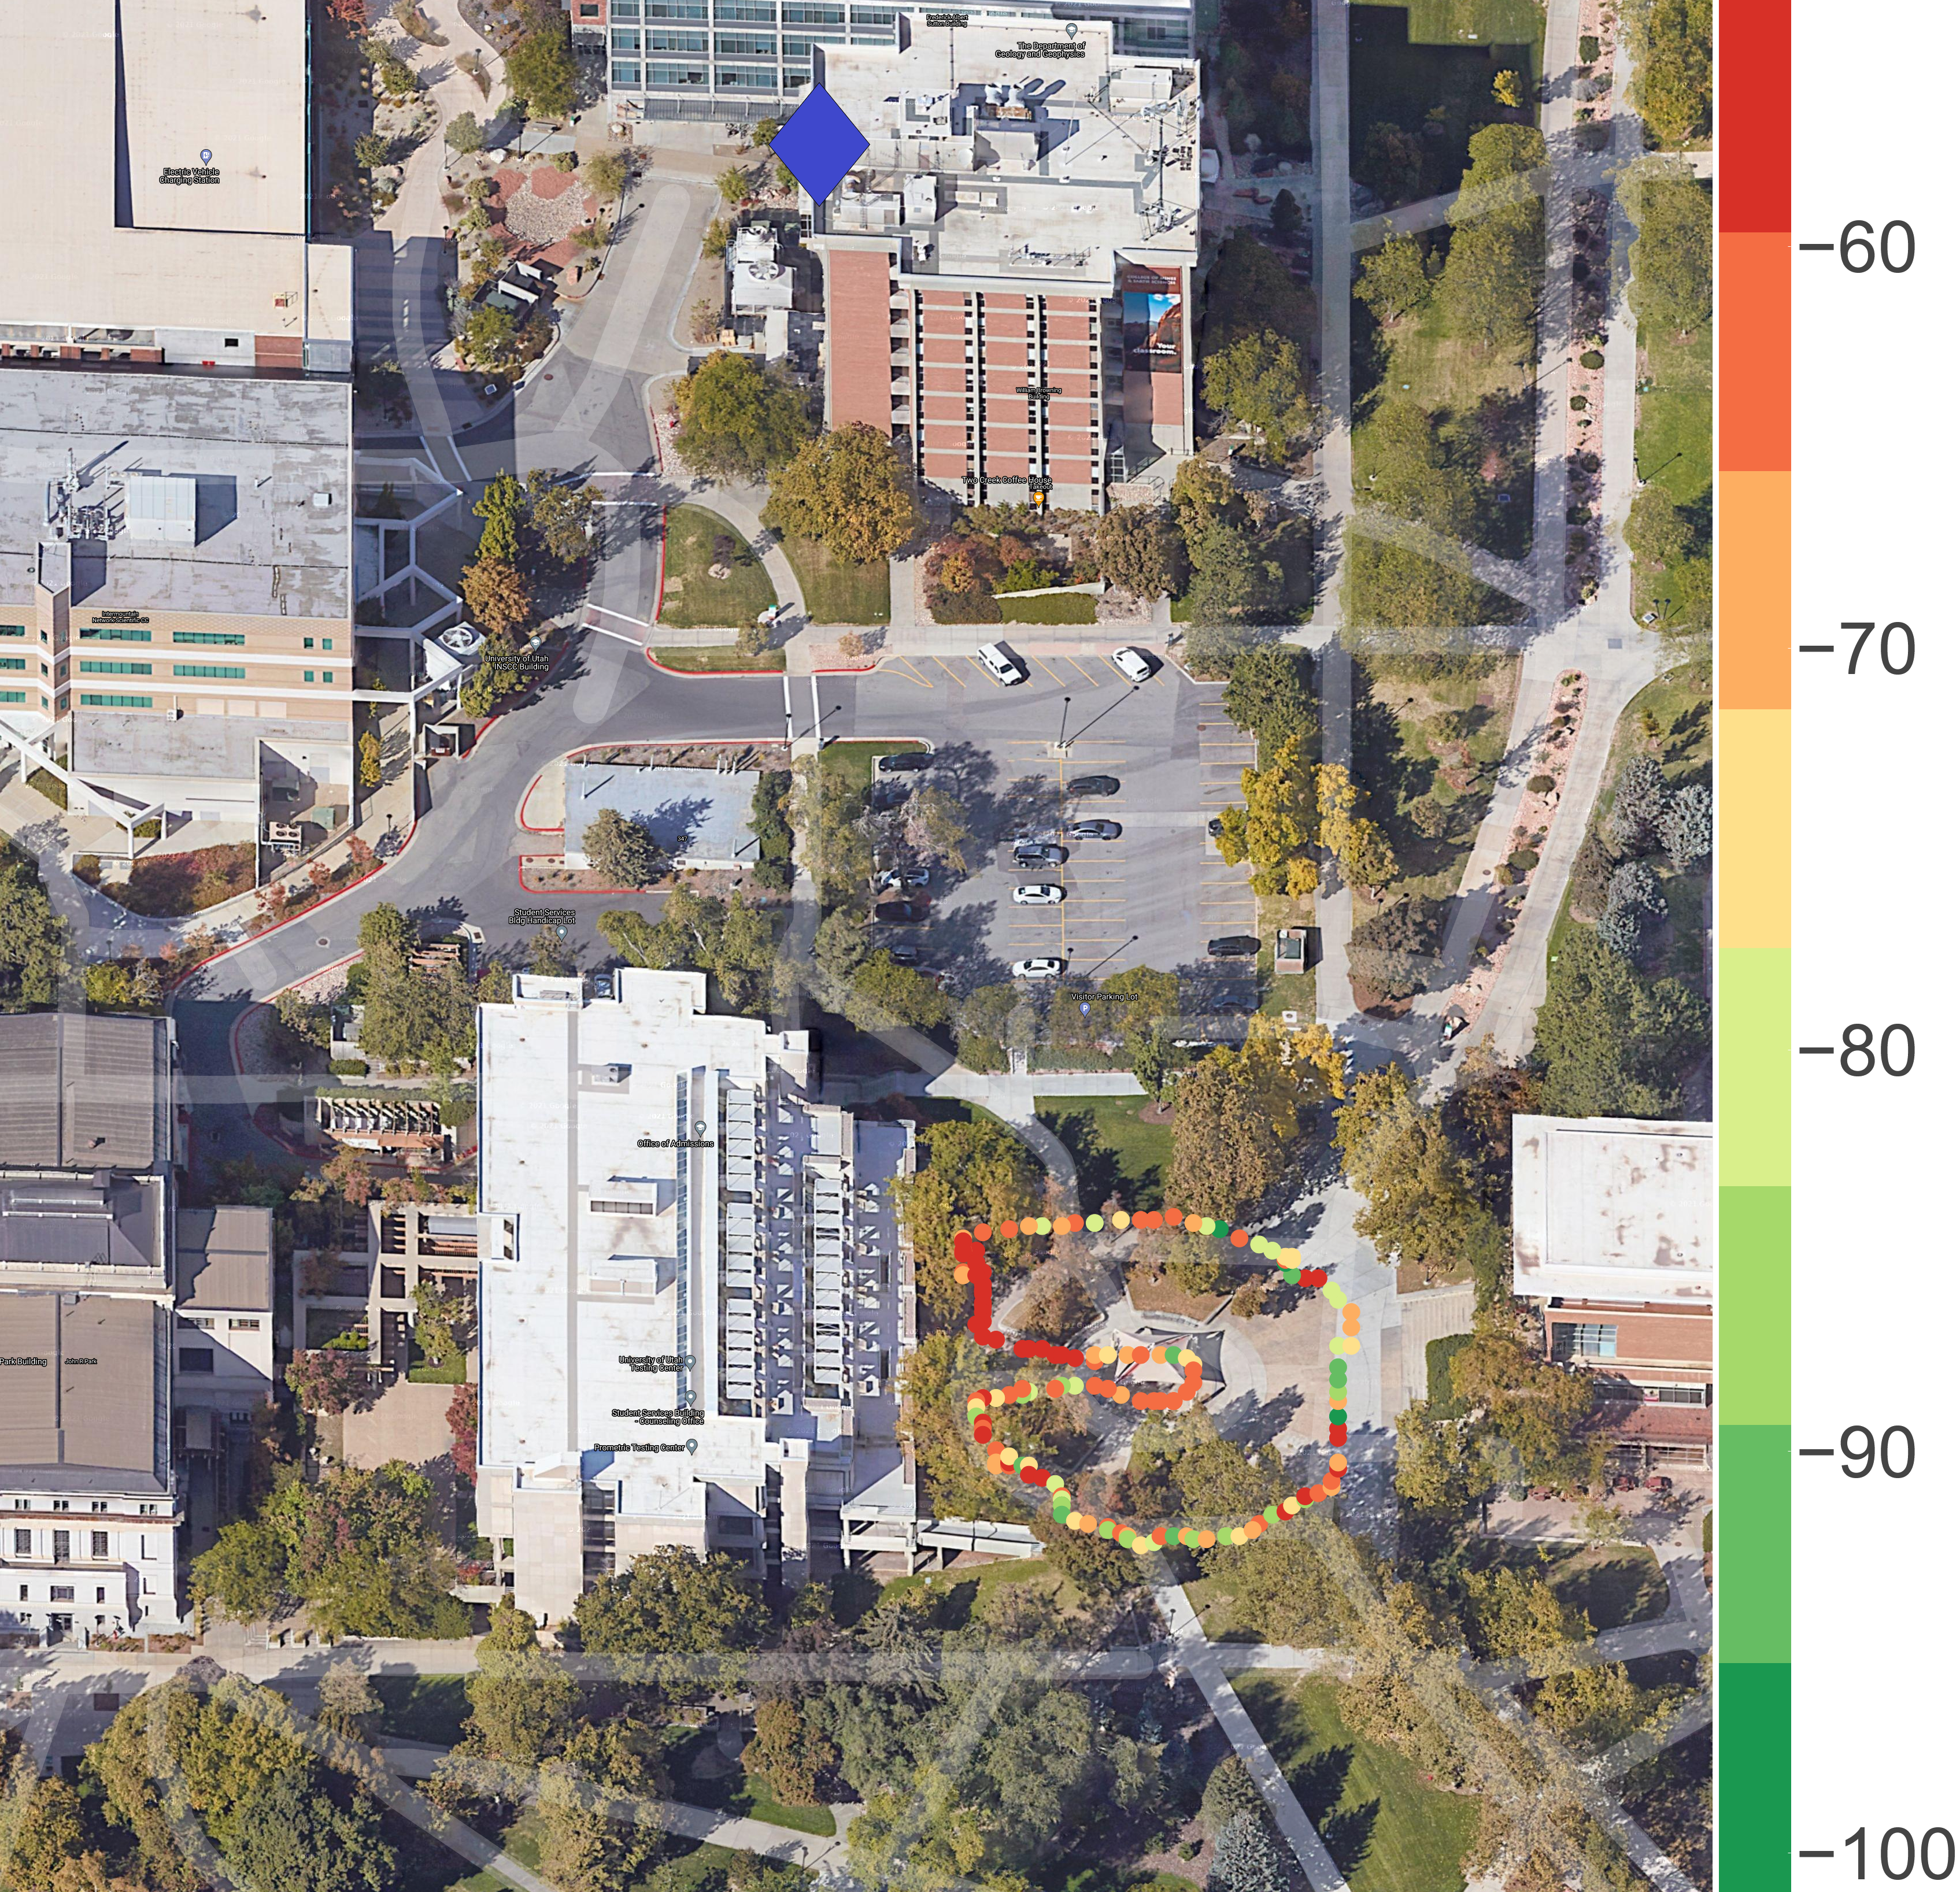
\includegraphics[width=1.0\linewidth]{figs/Rx_Power_Map_Foliage.png}
         \caption{Urban Foliage}
         \label{F4b}
     \end{subfigure}
     \begin{subfigure}{0.333\linewidth}
         \centering
         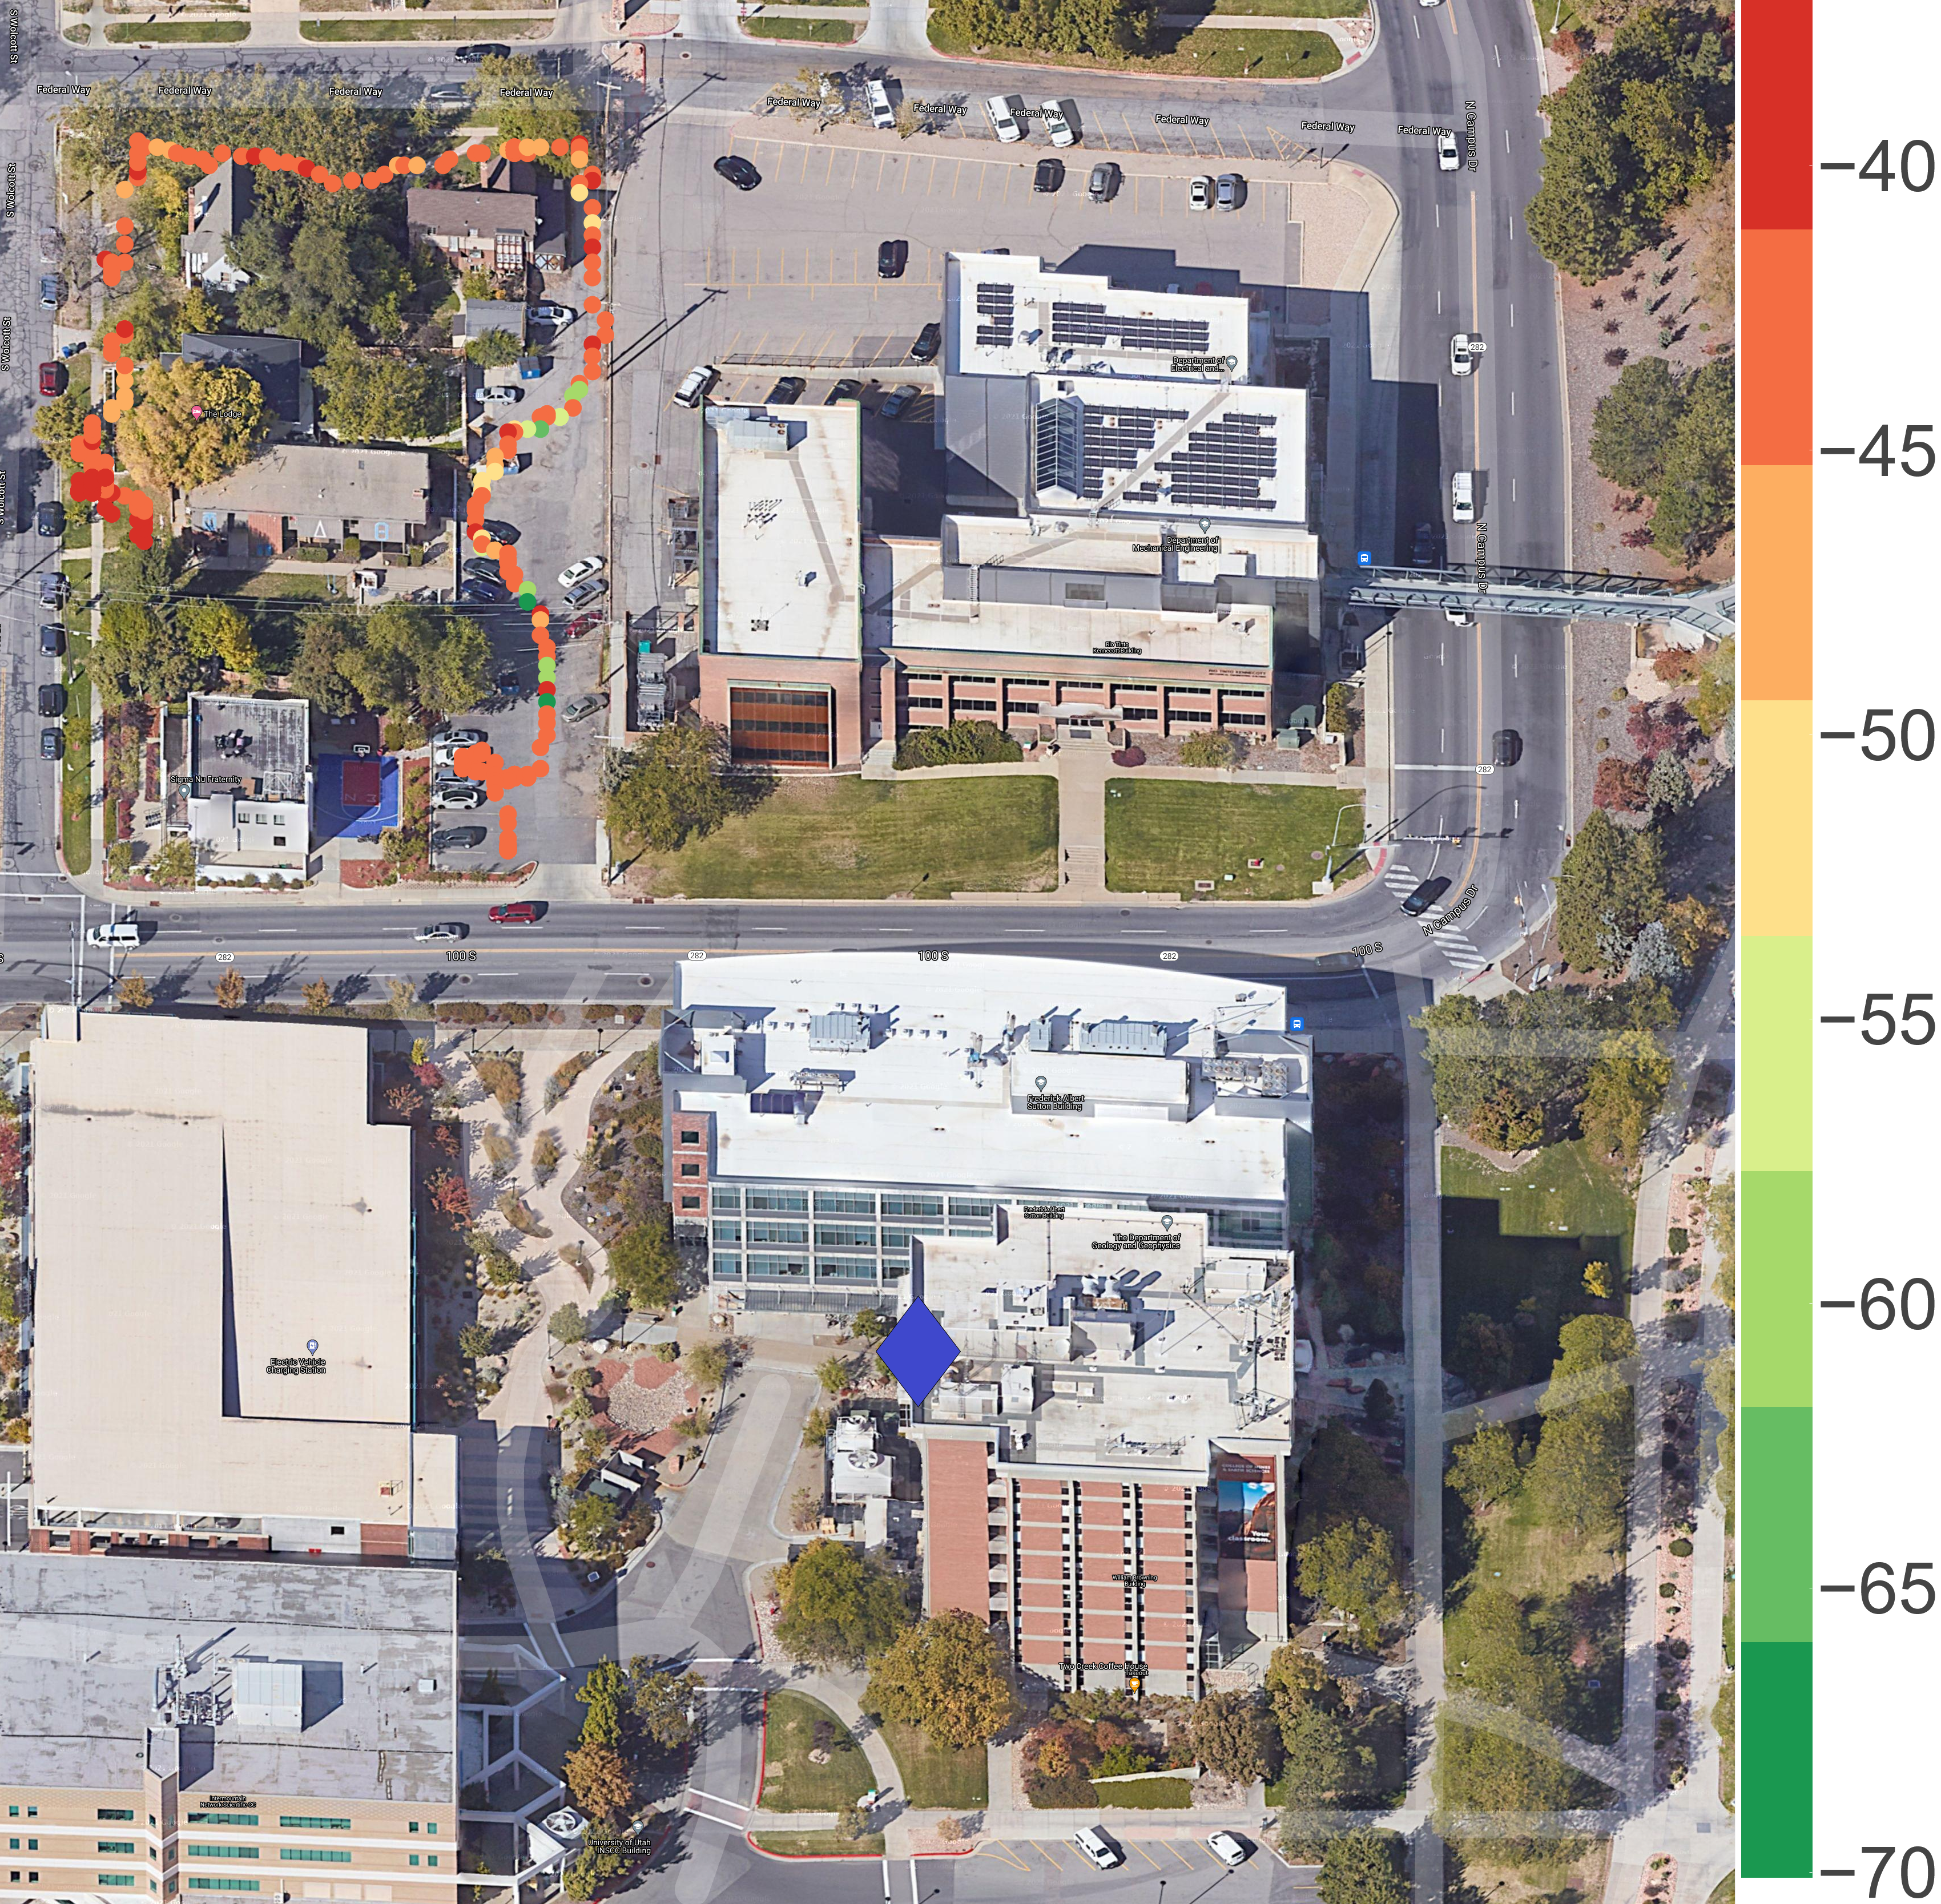
\includegraphics[width=1.0\linewidth]{figs/Rx_Power_Map_Suburban.png}
         \caption{Suburban Neighborhood}
         \label{F4c}
     \end{subfigure}
     \vspace{-2mm}
     \caption{The illustrations of the pathloss values superimposed on a Google Hybrid map of the sites under analysis for urban campus (Rx on minivan), urban foliage (Rx on cart), and suburban neighborhood (Rx on cart), respectively. The dots with heat-map color palette values denote Rx locations as it is driven/pushed around, and the purple diamond denotes the fixed Tx location.}
     \label{F4}
     \vspace{-6mm}
\end{figure*}

To analyze the spatial decoherence characteristics of \SI{28}{\giga\hertz} signals in vehicular communication settings, we employ the SAGE algorithm \cite{SAGE1} to extract the complex attenuation ($\alpha$), delay ($\tau$), and Doppler frequency ($\nu$) of the $M$ specular paths arriving at the Rx while traversing a particular route onsite. Since obtaining the exact high-resolution maximum likelihood estimate of this parameter vector ($\mathbf{\theta}{=}[\alpha_{i},\tau_{i},\nu_{i}]^{\intercal},i{=}1,2,{\dots},M$) directly involves prohibitively large computation times \cite{SAGE1}, the SAGE algorithm---an EM variant---solves for an approximate estimate of $\mathbf{\theta}$ via iterative executions of the E-step which computes the expectation of the log-likelihood given the observations and the previous estimate (using the Forward-Backward algorithm) and the M-step which computes the current estimate by maximizing over the E-step result (solved in closed-form). This iterative execution occurs until convergence, i.e., the parameter values do not change with iterations beyond a threshold ($\epsilon{=}10^{-6}$). Lastly, using these estimates, we plot the RMS delay- and direction-spread of the received signals while traversing the urban campus route around President's Circle.
\vspace{-5mm}

\section{Conclusion}\label{S5}
\vspace{-2mm}
We discuss the development of a fully autonomous robotic beam-steering platform coupled with a sliding correlator channel sounder, well-suited for a \SI{28}{\giga\hertz} V$2$X measurement campaign on the NSF POWDER testbed. Corroborated onsite, our beam-alignment system demonstrates superior performance vis-\`{a}-vis geo-positioning accuracy, alignment reliability, and tracking response times; also, our design offers cost and computational advantages over electronic beam-steering approaches. Processing the recorded power-delay profiles via custom heuristics on noise elimination and thresholding, we conduct pathloss evaluations against ITU M$.2135$ and $3$GPP TR$38.901$ urban macro-cellular standards. More importantly, the continuous series of measurements facilitated by our system design enables V$2$X spatial consistency studies under the effects of Tx-Rx distance, relative alignment, and relative velocity. Future extensions to this work revolve around empirical validations of widely-used outdoor mmWave channel models. Additional evaluations include elevation-delay dependence studies, analyses of cluster inter-arrival times, and peak-power distribution studies. These evaluations are further enhanced with Wireless InSite calibrated ray-tracing simulations on the terrain and structural profiles of the POWDER site.
\vspace{-5mm}

\bibliographystyle{IEEEtran}
\bibliography{IEEEabrv,main} 

\end{document}